\documentclass[12pt,a4paper,UTF8]{article}
\usepackage{ctex} % Chinese support
\usepackage{graphicx} % Insert images
\usepackage{subfigure}
\usepackage{float}
\usepackage{listings} % Print source code
\usepackage{color} % Color support
\usepackage{booktabs} % Professional table support
\usepackage{pdflscape} % Landscape pages support in PDF
\usepackage{hyperref} % Hypertext links support for cross-referencing
\usepackage{amsmath,mathtools}
\usepackage{ulem} % strikethrough

% Customize hyperref format (it's set to no special format here)
\hypersetup{hidelinks}

% Declare directories to search for graphics files for graphicx
\graphicspath{{figures/}}

% Define source code style for listings
\lstdefinestyle{verilog-style}{
	language=Verilog,
	basicstyle=\ttfamily\footnotesize,
	keywordstyle=\bfseries\color[rgb]{0, 0, 1},
	identifierstyle=\color[rgb]{0.5, 0.3, 0.1},
	stringstyle=\color[rgb]{0.6, 0.1, 0.1},
	commentstyle=\itshape\color[rgb]{0.05, 0.5, 0.05},
	backgroundcolor=\color[gray]{0.95},
	numbers=left,
	numbersep=5pt,
	numberstyle=\color[gray]{0.6},
  breaklines=true,
  escapeinside=``
}

\newcommand{\reporttitle}[2]{
  \LARGE\textsf{#1}\quad\underline{\makebox[12em]{#2}}
}

\newcommand{\reportinfo}[2]{
  \large\makebox[4em]{\textsf{#1}}\quad\underline{\makebox[18em]{#2}}
}

\begin{document}
\begin{titlepage}
  \centering
  \vspace*{\fill}
  {\Huge\textsf{数字电路与数字系统实验}} \\ [100pt]
  \reportinfo{实验名称}{exp11 字符输入界面} \\ [10pt]
  \reportinfo{院系}{计算机科学与技术系} \\ [10pt]
  \reportinfo{学生姓名}{} \\ [10pt]
  \reportinfo{学号}{} \\ [10pt]
  \reportinfo{班级}{数字电路与数字系统实验1班} \\ [10pt]
  \reportinfo{邮箱}{} \\ [10pt]
  \reportinfo{实验时间}{2020 年 11 月 8 日} \\ [10pt]
  \vspace*{\fill}
\end{titlepage}
\tableofcontents
\newpage

\section{实验目的}
\begin{itemize}
  \item 了解字模点阵相关的知识
  \item 综合运用存储器、键盘、显示器的相关知识,
        学习多个模块之间的交互和接口设计
  \item \sout{速成大型Verilog程序的debug能力}
\end{itemize}


\section{实验原理}
\begin{itemize}
  \item 字模点阵可以存储在存储器中,
        然后通过扫描输出到显示器对应像素点上
  \item 读写存储器的原理(详见实验7)
  \item 键盘输入的原理(详见实验8)
  \item VGA控制模块的相关原理(详见实验9)
\end{itemize}


\section{实验环境/器材}
\begin{itemize}
  \item Quartus编辑器和DE10-Standard开发平台
  \item FPGA开发板
  \item 带有PS/2接口的键盘
  \item 带有VGA接口的显示器
\end{itemize}


\section{模块结构设计}
实现字符输入交互界面是一个大工程,我们需要综合运用存储器、
键盘控制、显示器输出等多个模块的内容。如果糅合在一起编写,
直到写完之后再去测试,这会使debug变得非常困难。所以我们必须
把这个大工程拆分成几个子工程,实现完一部分就测试一部分,保证
先前编写的模块不出问题,再去实现下一部分。

``把大工程拆分成子工程'',这里的``子工程''指的是几个
拥有共同上层模块的模块的集合。我们把这个共同的上层模块称为
``子工程的顶层模块'',该模块也包含在子工程中。每个子工程
的输出可以传递给大工程进行最终输出,也可以作为输入参数传递
给另一个子工程。每个子工程可以调用(包含)相同的模块,
即它们可以有交集。但是它们必须是一级驱动下一级的,
即一个(或多个)子工程的输出作为参数传递给下一个
子工程,使其根据该参数进行输出,依次类推。

我们划分子工程的目的是为了debug,即每个子工程的输出
必须能在\linebreak[4]
FPGA开发板或显示器等器件上显示出来,并保持一段
时间不变,使得我们可以用肉眼观察输出情况。所能拆分的
子工程越多,debug就越容易。但是对于本实验而言,只拆分出
两个子工程最为合适。因为关于键盘输出,我们已经在实验8
中大致实现了,只要稍作修改并观察按键输出是否正确即可;
而关于显示器方面,显示器所要输出字符的ASCII码
都保存在一个30$\times$70的存储器里,对它进行修改
需要在同一个always块中实现,无法拆分出更多模块
(子工程)。扫描显示屏幕的模块也可以作为一个子工程,
但是该模块已经在实验9的题目中提供了,不需要我们进行
调试,所以我们把它合并到了显示器相关的子工程中。

因此,我们最终把本实验的工程拆分为两个
子工程,一个子工程输出键盘按键的ASCII码,以及CapsLock、
Shift、方向键等控制键的按键情况,另一个子工程根据这些
输出改写显示屏幕的存储器,然后反馈到显示器上。

模块调用层次结构如下:
\begin{figure}[H]
  \centering
  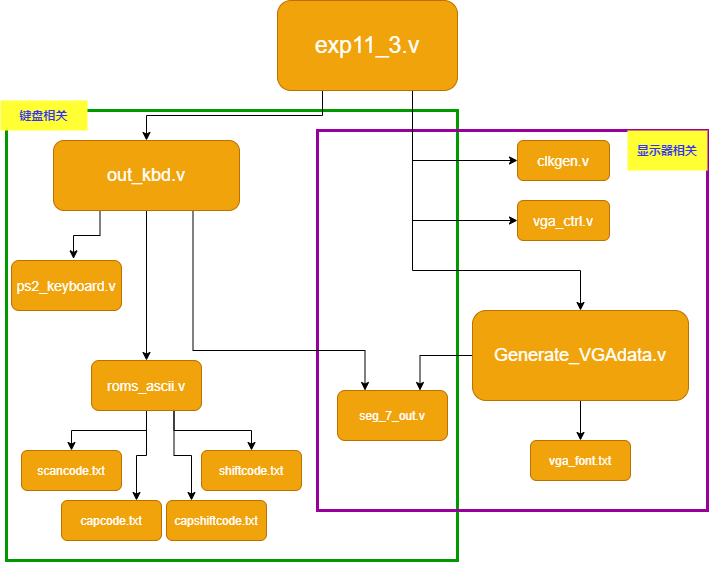
\includegraphics[width=1\textwidth]{code_structure.PNG}
  \caption{模块层次结构}
  \label{struct}
\end{figure}

\section{实验步骤/过程}
\subsection{键盘控制部分}
为了称呼方便,我们把键盘分为三种键,定义如下:
\begin{description}
  \item[有效字符键] 按下后屏幕上会增加相应字符的键,
        如字母、数字、符号等。
  \item[无效字符键] 按下后屏幕输出以及光标都不发生
        改变的键,如CapsLock、Shift、\mbox{F0$\sim$F12}等
  \item[非字符屏幕变化键] 除去有效字符键之外,按下后会使
        屏幕输出或光标变化的键。本实验中只实现了左方向键、
        右方向键、回车键和退格键,可扩展(如上下方向键、
        delete键等)。
\end{description}

对于无效字符键,在本实验中只有大小写与其相关,
而其他子工程可以通过ASCII码来判断当前需要输出的
是大写还是小写,所以我们可以在键盘子工程内处理
无效字符键的问题,不需要把它作为键盘子工程的输出。
因此,我们只需要把有效字符键(结合此时无效字符键
的按键情况)的ASCII码和非字符屏幕变化键作为
键盘子工程的输出即可:

为了便于debug,我一开始另建了一个工程专门来测试
键盘部分,把所有用于debug的变量都输出到FPGA开发板上
进行观察,如按键扫描码等。在把键盘子工程与其他子工程
合并之后,仍然保留下来的输出有如下几个信号:
\begin{itemize}
  \item 当前按键的ASCII码,输出到七段数码管
        \mbox{HEX1}和\mbox{HEX0}上。
  \item 无效字符键,输出到\mbox{LEDR[3:0]}
        (一个键对应一个信号灯)
  \item 非字符屏幕变化键的编号,输出到\mbox{LEDR[7:5]}
        (3个二进制位,表示编号0$\sim$7)
  \item 非字符屏幕变化键的按键信号(按任意该类键即触发有效),
        输出到\mbox{LEDR[9]}
\end{itemize}

本实验的键盘模块与实验8不同之处在于:我们需要处理
方向键的扫描码,这些键的通码由两个8位二进制串组成,
其中第一个8位二进制串用十六进制表示为E0。我们需要修改
实验8的键盘控制代码,使其能够处理这样的扫描码。

处理思路如下:
\begin{lstlisting}[style=verilog-style]
/*`注:此always块中的时钟信号频率很快,同一个扫描码会被多次读取`*/
if (ready) begin
  if (/*`扫描码读到F0`*/) begin
    /*`接下来的按键无效(在读完这个F0之前不做其他任何事)`*/
    /*`把非字符屏幕变化键的按键信号变为无效`*/
    /*`有效的扫描码置为零(此时扫描码为无效字符)`*/
  end else begin
    if (/*`刚刚读完F0,现在是紧接着F0的断码`*/) begin
      /*`接下来的按键有效(指完全读完这个断码以后)`*/
      /*`过一段时间(0.1秒)再读下一个扫描码,以保证下一个读到的是通码`*/
      /*`如果此时的断码对应一个无效字符键的话,那么设置此键的按键状态`*/
    end else if (/*`按键有效`*/) begin
      if (/*`扫描码读到E0`*/) begin
        /*`下一次读扫描码如果还是同一个E0,那么不做其他任何事`*/
        /*`有效的扫描码置为零(此时扫描码为无效字符)`*/
      end else begin
        /*`这部分用于处理三种键(有效字符键、`
        `无效字符键和非字符屏幕变化键)的通码`*/
        if (/*`刚刚读完E0,现在是紧接着E0后面的8位二进制扫描码`*/) begin
          /*`改变此if块的条件变量的状态(下一次读扫描码时,那时的前一个`
          `读取的扫描码,也即本次读取的扫描码,不是E0,而是紧接着E0后面的`
          `8位二进制扫描码,所以不应该进入此if块)`*/
          if (/*`扫描码读到F0,说明是非字符屏幕变化键的断码`*/) begin
            /*`与读到F0做同样的操作`*/
          end else begin
            /*`此时读到的是方向键的通码,根据扫描码进行相应设置`*/
            /*`我们把Shift和ctrl归为无效字符类,但是这两个键也有`
            `E0+通码的情况,所以也在这里进行判断和设置`*/
          end
        end else begin
          if (/*`无效字符键的通码`*/) begin
            /*`有效的扫描码置为零(此时扫描码为无效字符)`*/
            /*`根据扫描码进行相应按键设置`*/
          end else begin
            /*`有效的扫描码置为当前的扫描码`*/
          end
        end
      end
    end
  end
  nextdata_n <= 0; 
end else nextdata_n <= 1;
\end{lstlisting}

我们实现完键盘子工程后,下载到FPGA开发板上进行测试。
观察FPGA开发板上相应信号的输出值,在确保无误之后,
就可开始下一个子工程的模块实现。

\subsection{显示器部分}
如何扫描显示已经在题目pdf中讲的很清楚了,只要
根据图\ref*{scan_display}用assign语句进行赋值
即可。
\begin{figure}[H]
  \centering
  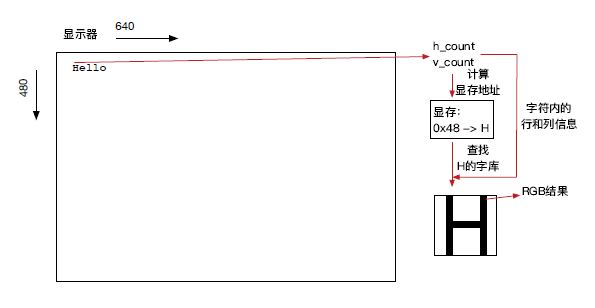
\includegraphics[width=1\textwidth]{scan_display.JPG}
  \caption{扫描显示}
  \label{scan_display}
\end{figure}

我们主要描述如何设计显示屏幕的存储器。我对屏幕显示设计如下:
第一行输``Hello, world'',第二行为空行,我们输入的字符
所能出现的位置从屏幕上第三行开始。默认初始屏幕的第三行会有
命令提示符``myshell$>$'',光标位于命令提示符之后。键盘的输入
对光标所在的位置进行填充字符或修改字符。左右方向键移动光标,向前
最多能够移动到命令提示符之后,向后最多能够移动到有输入的最后
一行末尾的非空字符后。我们把这个``有输入的最后一行末尾的非空
字符后''的位置记为L。对于回车键,无论光标位于何处,都会针对
位置L进行换行,换行后在行首填充命令提示符,然后把光标挪至
命令提示符之后。对于退格键,只有当光标位于位置L时才会删除
光标前一个字符,否则不进行任何操作。当光标和位置L都处于屏幕
最右下角时,输入字符会使得屏幕清空(第一行和第二行不改变),
新输入的字符出现在第三行的第一个位置,光标停留在该位置之后。

下面来解释一下关于显示屏幕存储器的庞大的always块:
\begin{lstlisting}[style=verilog-style]
if (/*`键盘无有效输入`
  `(未按下非字符屏幕变化键且键盘输出的ASCII码为0)`*/) begin
  /*`光标闪烁`*/
end else if (/*`按下的是非字符屏幕变化键`*/) begin
  /*`光标常亮(白色)`*/
  /*`根据按下的非字符屏幕变化键,进行相应操作(case语句选择执行)`*/
  /*case left*/: begin
    if (/*`光标不在命令提示符后一格`*/) begin
      if (/*`光标在某行第一格`*/) begin
        if (/*`光标不在第三行`*/) /*`光标移至上一行的最后一格`*/
      end else /*`光标左移一格`*/
    end
  end
  /*case right*/: begin
    if (/*`光标在位置L之前`*/) begin
      if (/*`光标在某行的最后一格`*/) begin
        /*`光标移至下一行的第一格`*/
      end else /*`光标右移一格`*/
    end
  end
  /*case enter*/: begin
    if (/*`位置L在屏幕的最后一行`*/) begin
      /*`清空屏幕,然后输出命令提示符`*/
    end else /*`换行并输出命令提示符`*/
  end
  /*case backspace*/: begin
    if (/*`光标在位置L处`
      `且光标不在第三行第一格`
      `且光标不在命令提示符后一格`*/
    ) begin
      if (/*`光标在某行第一格`*/) begin
        /*`删除该格字符并把光标移至上一行的最后一格`*/
        /*`更新位置L`*/
      end else begin
        /*`删除该格字符并把光标左移一格`*/
        /*`更新位置L`*/
      end
    end
  end
  default: /*`光标位置不变`*/
end else begin
  /*`此时按下的是有效字符键`*/
  if (/*`光标在某行的最后一格`*/) begin
    if (/*`光标在最后一行`*/) begin
      /*`清空屏幕,然后输出按下的字符键`*/
    end else begin
      /*`换行输出字符`*/
      /*`判断是否更新位置L`*/
    end
  end else begin
    /*`输出字符并移动光标`*/
    /*`判断是否更新位置L`*/
  end
end/*``*/
\end{lstlisting}

这样,我们就完成了显示器相关的子工程。把两个子工程
合并成一个大工程,下载到FPGA开发板上运行,测试成功即
本实验完成。


\section{测试方法和实验结果}
直接下载到FPGA开发板上运行,用键盘和显示器进行测试,
各项功能都成功实现:
\begin{figure}[H]
  \centering
  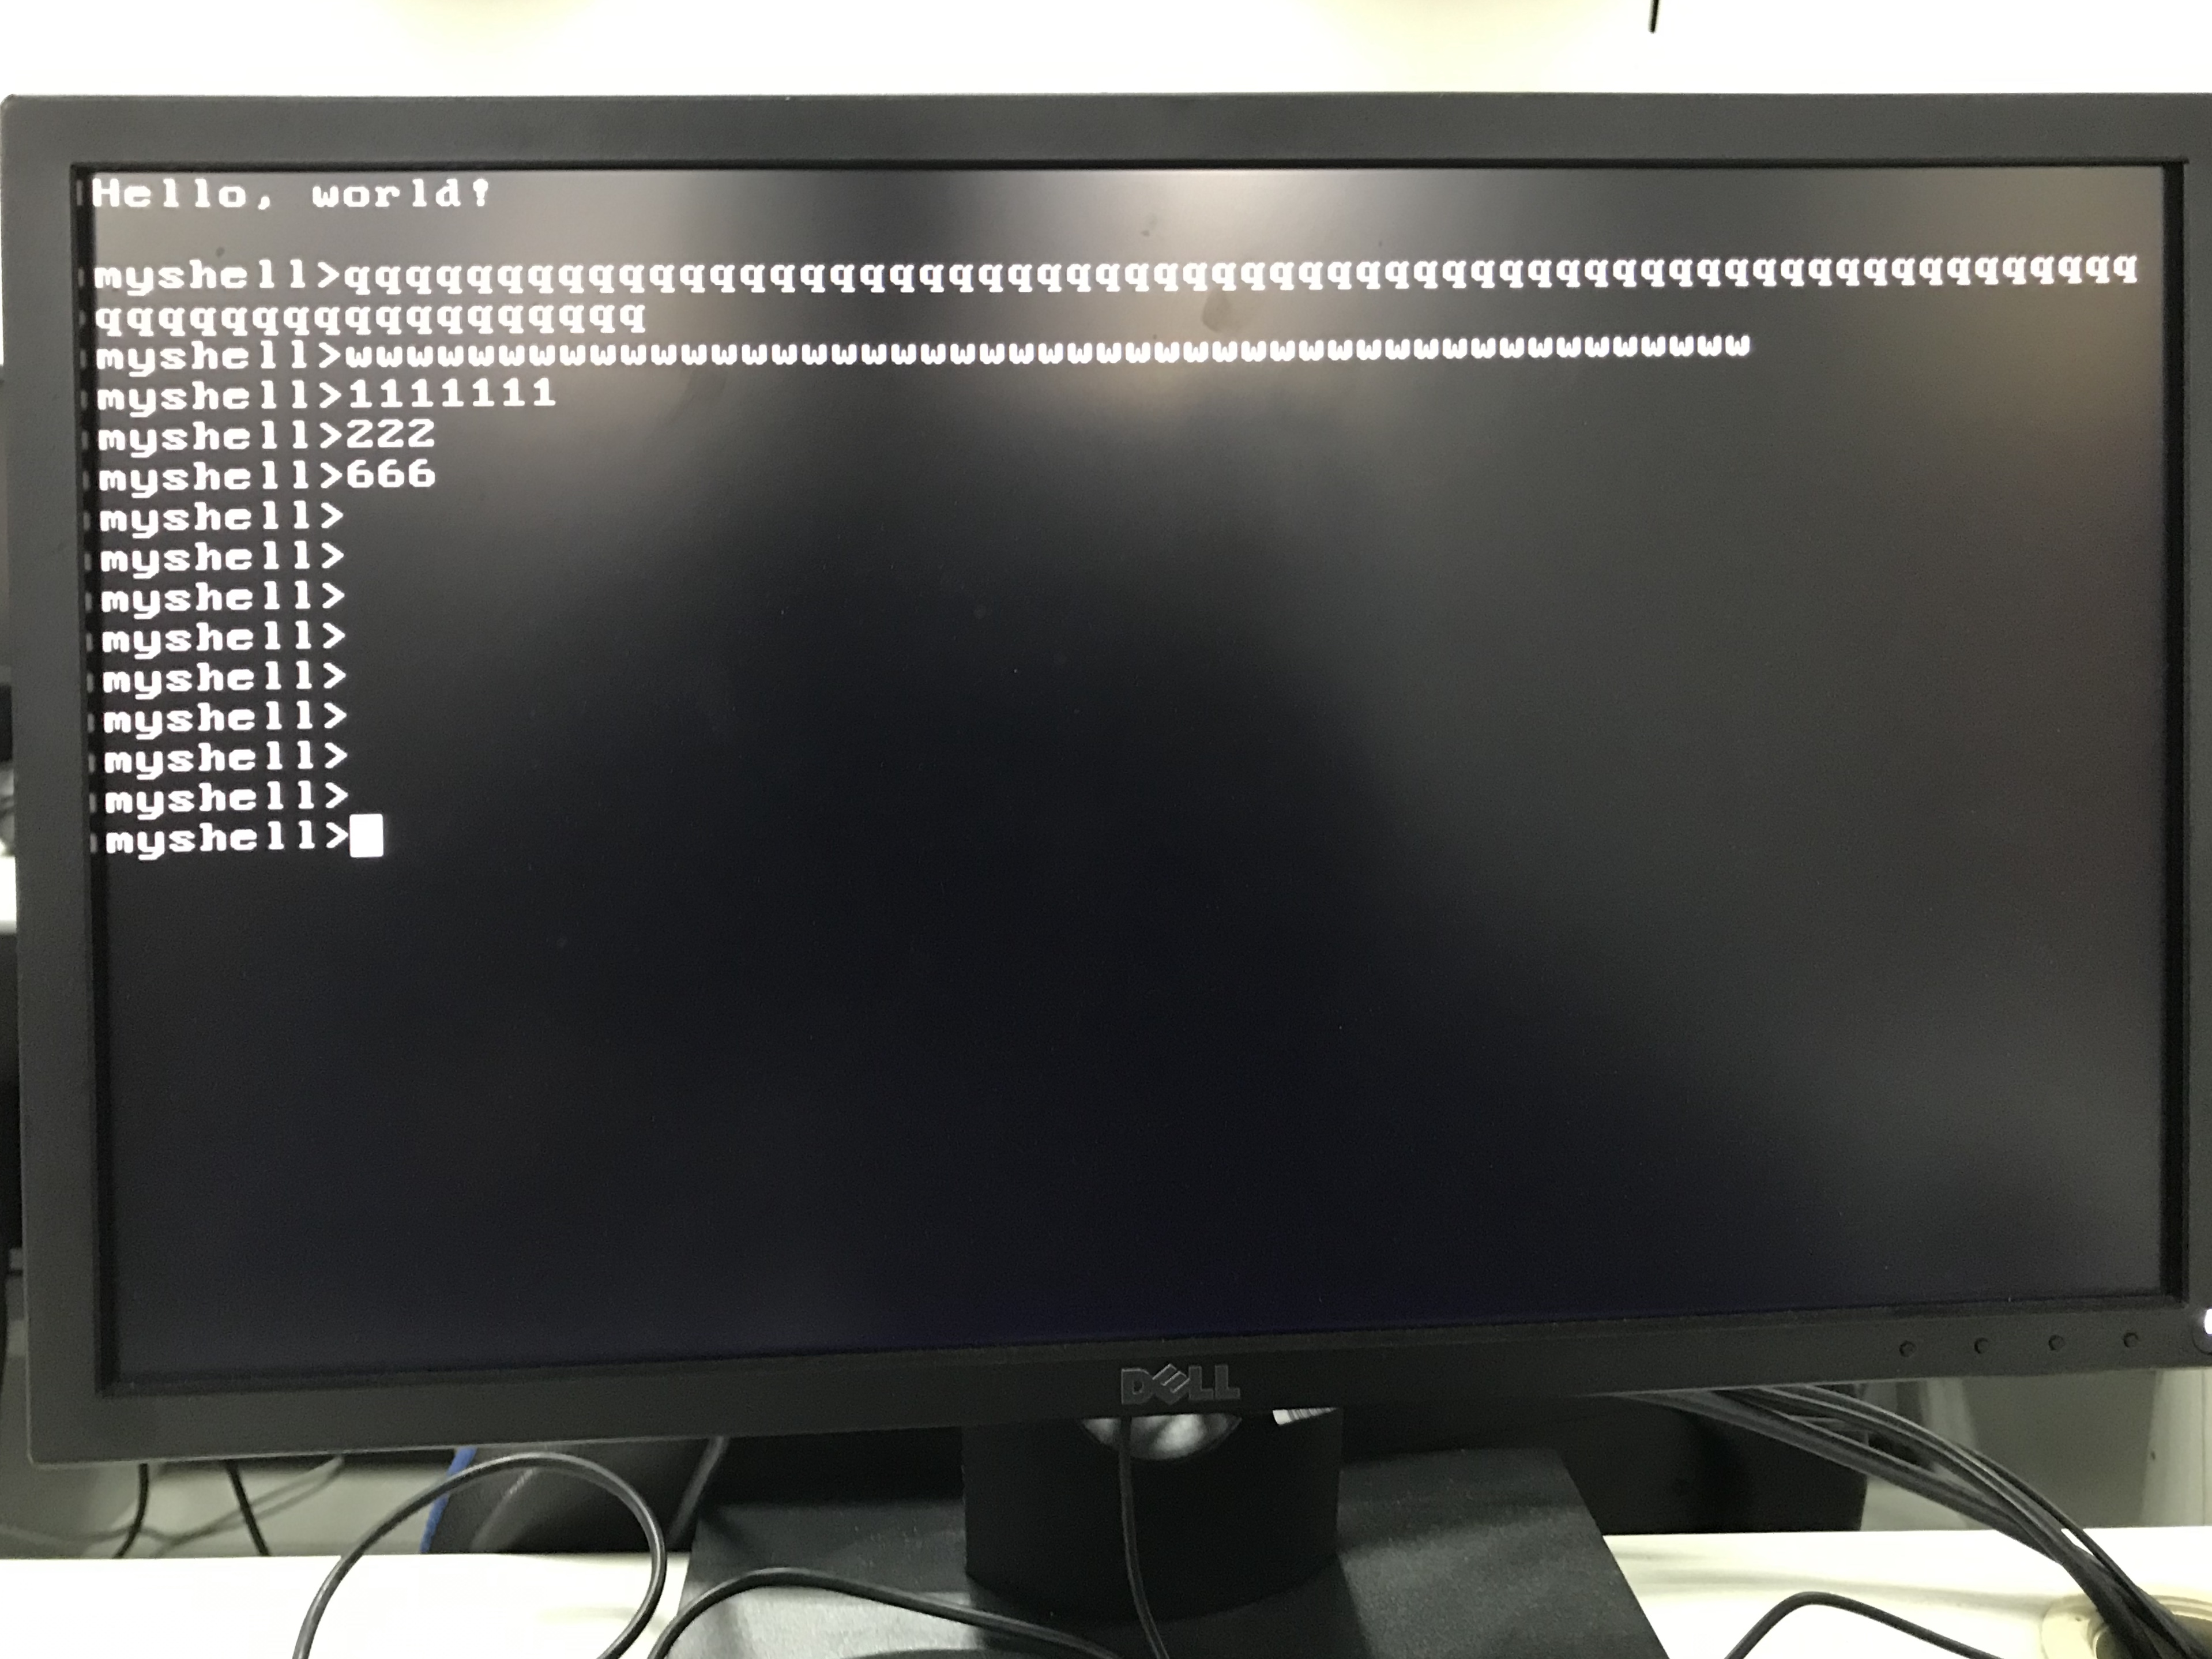
\includegraphics[width=1\textwidth]{fpga.JPG}
  \caption{屏幕显示}
  \label{fpga}
\end{figure}


\section{遇到的问题及解决办法}
\begin{itemize}
  \item 字模点阵的列数为9,所以其存储器的列数下标索引必须
        是4位的变量,位数过宽可能会出一些奇奇怪怪的问题
  \item 用FPGA开发板上的按钮进行屏幕清零会清零失败(存储器
        没有更新为0),可能是因为扫描的时钟和屏幕输出的时钟
        不同步
\end{itemize}


\section{得到的启示}
在设计一个大工程之前,先要考虑清楚各个模块的接口,
以便划分成几个子工程,有助于debug的进行。


\section{意见和建议}
\sout{相比于前几个实验,这次实验代码量暴涨,而且扩展要求难度
  有点大,要求完成的扩展功能数量有亿点点多$\cdots$稍微降低点要求吧
  我太难了呜呜呜}

\end{document}